\documentclass[tikz,border=10pt]{standalone}
% Scale s = 0.022663 cm/px (from STYLE METRICS); origin at O
\begin{document}
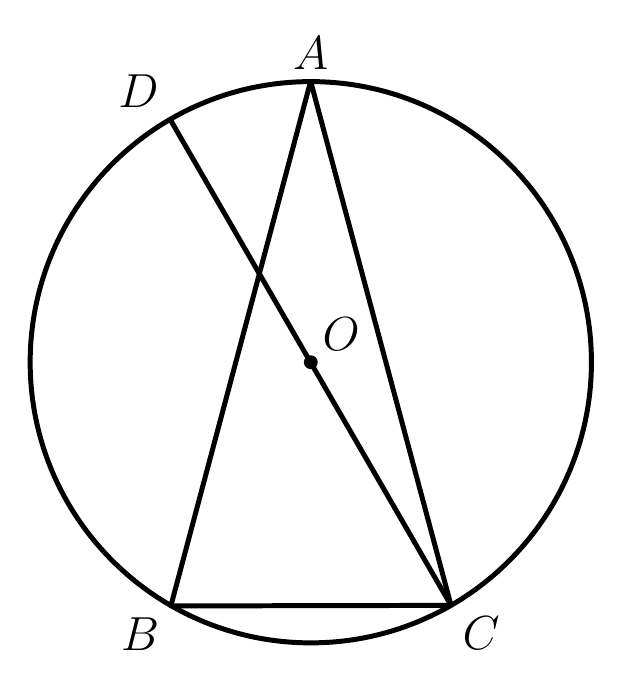
\begin{tikzpicture}[line join=round, line width=1.8pt, font=\fontsize{19}{22.8}\selectfont]
  % Key points (cm), y flipped, relative to O
  \coordinate (O) at (0,0);
  \coordinate (A) at (-0.002,3.568);
  \coordinate (B) at (-1.777,-3.095);
  \coordinate (C) at (1.781,-3.088);
  \coordinate (D) at (-1.786,3.084);

  % Circle of radius 157.27 px
  \draw (O) circle (3.564);

  % Triangle ABC
  \draw (A) -- (B) -- (C) -- cycle;
  % Diameter DC through O (solid)
  \draw (D) -- (C);

  % Centre dot
  \fill (O) circle (2.5pt);

  % Labels
  \node[above right] at (O) {$O$};
  \node[above] at (A) {$A$};
  \node[below left] at (B) {$B$};
  \node[below right] at (C) {$C$};
  \node[above left] at (D) {$D$};
\end{tikzpicture}
\end{document}